\chapter{Particle Flow Calorimetry and Linear Collider Detectors}
\label{chap:reconstructionchain}

\chapterquote{I am fond of pigs.  Dogs look up to us.  Cats look down on us.  Pigs treat us as equals.}
{Winston Churchill}

\section{Particle Flow Calorimetry}

The premise of particle flow calorimetry is to measure the energy of individual particles in detector using the sub-detector that offers the best energy resolution.  For particle collider experiments, the biggest contrast to tradition calorimetry is that the energy of charged particles is measured using the curvature of the tracks they produce in the tracker instead of measuring their energy in calorimeters.  The energy resolution for these charged particles is significantly better when using the particle flow approach to calorimetry, which leads to exceptionally good jet energy resolutions that can be used for characterising multi-jet final states in physics processes of interest at the linear collider experiment.  Furthermore, these energy resolutions are highly beneficial for quantifying those final states involving charged leptons and missing momentum, due to the presence of neutrinos.

\begin{figure}
\centering
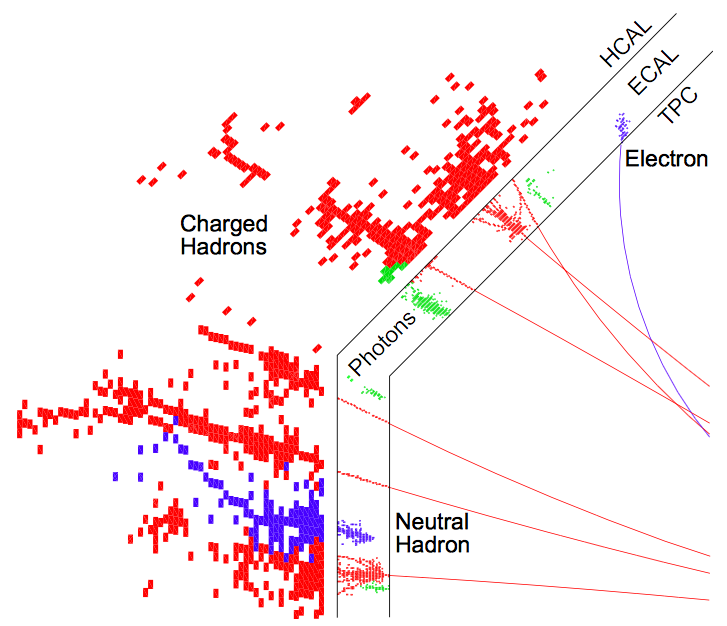
\includegraphics[width=0.5\textwidth]{LCDetectorsAndPFlow/Plots/Pictures/PFlow.png}
\caption[A typical simulated 250 GeV jet in the CLIC\_ILD detector, with labels identifying constituent particles.  Image taken from  \cite{arXiv:1209.4039}.]{A typical simulated 250 GeV jet in the CLIC\_ILD detector, with labels identifying constituent particles.  Image taken from  \cite{arXiv:1209.4039}.}
\label{fig:particleflowpic}
\end{figure} 

Particle flow calorimetry is challenging to put into practice as it requires a precise reconstruction for all long-lived particles within a detector.  Charged particles have their energy measurements taken from the curvature of the track they transverse, but they also produce calorimetric energy deposits, as shown in figure \ref{fig:particleflowpic}, and if both energy measurements are included the energy of the charged particle will be double counted.  Therefore, the precise reconstruction has to associate charged particle tracks to their corresponding calorimetric energy deposits.  This can only be realised by using calorimeters with fine segmentation so that it is possible to resolve individual particle showers within them.  This is the basis for the design of the linear collider calorimeters.  While double counting of energy of charged particles is possible, it is also possible to omit the energy measurements of neutral particles.  This occurs if a neutral particle calorimetric energy deposit, which is the only energy measurement produced for a neutral particle, is incorrectly associated to a track.  In such a case the calorimetric energy deposit will not be used as the reconstruction believes the energy is from a charged particle and so will come from the track and the neutral hadron energy will be lost.  These two effects form the confusion contribution to the jet energy resolution, which acts to degrade the energy resolution of a particle flow calorimetry based detector.  

\begin{table}[h!]
\centering
\begin{tabular}{ l l l l l}
\hline
Jet  & Detector & Energy & Energy & Jet Energy \\
Component &  & Fraction & Resolution & Resolution Contribution \\
\hline
Charged & Tracker & $\sim 0.6 E_{j}$ & $10^{-4} \times E_{X^{\pm}}^{2}$ & $< 3.6 \times 10^{-5} \times E_{j}^{2}$ \\
Particles ($X^{\pm}$) & & & & \\
Photons & ECal & $\sim 0.3 E_{j}$ & $0.15 \times \sqrt{E_{\gamma}}$ & $0.08 \times \sqrt{E_{j}}$ \\
($\gamma$) & & & & \\
Neutral & HCal &$\sim 0.1 E_{j}$ & $0.55 \times \sqrt{E_{X^{0}}}$ & $0.17 \times \sqrt{E_{j}}$ \\
Hadrons ($X^{0}$) & & & & \\
\hline
\end{tabular}
\caption[The approximate fractions, energy resolutions and jet energy resolution contributions made by charged particles ($X^{\pm}$), photons ($\gamma$) and neutral hadrons ($X^{0}$).  Table taken from \cite{arXiv:0907.3577}.]{The approximate fractions, energy resolutions and jet energy resolution contributions made by charged particles ($X^{\pm}$), photons ($\gamma$) and neutral hadrons ($X^{0}$).  Table taken from \cite{arXiv:0907.3577}.}
\label{table:pflowjet}
\end{table}

The magnitude of the improvements offered by particle flow calorimetry can be explicitly seen when considering the different contributions to the measurement of jet energies, which is summarised in table \ref{table:pflowjet}.  After the decay of short lived particles approximately 60\% of the energy of a jet is carried in the form of charged particles, 30\% in the form of $\gamma$s and 10\% in the form of neutral hadrons.  A negligible amount of energy is also carried in the form of invisible energy i.e. neutrinos.  In the traditional calorimetric approach $\gamma$s are measured within the ECal, with an energy resolution of $\sim 0.15 \times \sqrt{E_{\gamma}}$, and the remaining particles are measured in the HCal, with an energy resolution of $\sim 0.55 \times \sqrt{E_{X}}$.  This gives contributions to the jet energy, $E_{j}$, resolution of $\frac{0.08}{\sqrt{E_{j}}}$ and $\frac{0.46}{\sqrt{E_{j}}}$ from $\gamma$s and other particles respectively.  These add in quadrature to give a total jet energy resolution of $\frac{0.47}{\sqrt{E_{j}}}$.  In the particle flow paradigm the energy of charged particles is measured in the tracker, which has such a good energy resolution that its contribution to the jet energy resolution is negligible.  Therefore, contributions to the jet energy resolutions only come from $\gamma$s and from neutral hadrons, which when added in quadrature give a total jet energy resolution of $\frac{0.19}{\sqrt{E_{j}}}$.  This jet energy resolution is significantly better than that offered by the traditional calorimetric approach, however, it must be emphasised that this is an upper limit on the performance as the effect of confusion will degrade the jet energy resolution.  By applying sophisticated pattern recognition algorithms this confusion can be minimised and exceptional performance achieved.  While numerous approximations have been made in the above calculation it is clear that particle flow calorimetry has the potential to revolutionise detector deign for high energy physics experiments.

\section{Linear Collider Detectors}

All detector concepts for the linear collider have been purposely built to make particle flow calorimetry possible.  While there are a number of different concepts that are under consideration for both the ILC and CLIC one of the most prominent, and the focus of this work, is the International Large Detector (ILD).  The ILD detector, shown in figure \ref{fig:ild} realises very high spatial resolution for all sub-detector systems thanks to its highly granular calorimeters and central tracking system, all of which is encompassed within a 3.5 T magnetic field.  When combined with sophisticated pattern recognition software provided by PandoraPFA, particle flow calorimetry can be realised and the jet energy resolution can reach the goal of $3.8 \%$ which is required to allow separation of hadronic decays from W and Z bosons.  Details on each of the various sub-detector systems for ILD will now be discussed.

\begin{figure}
\centering
\subfloat[]{\label{fig:ild1}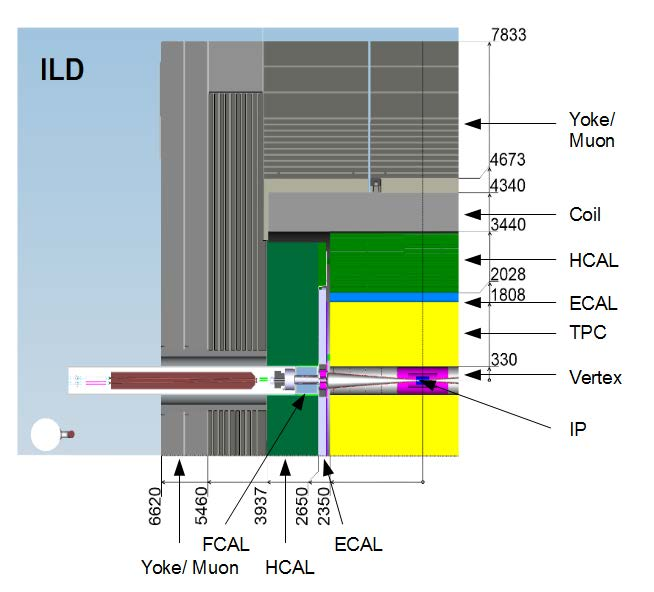
\includegraphics[width=0.5\textwidth]{LCDetectorsAndPFlow/Plots/Pictures/ILD.jpg}}
\subfloat[]{\label{fig:ild2}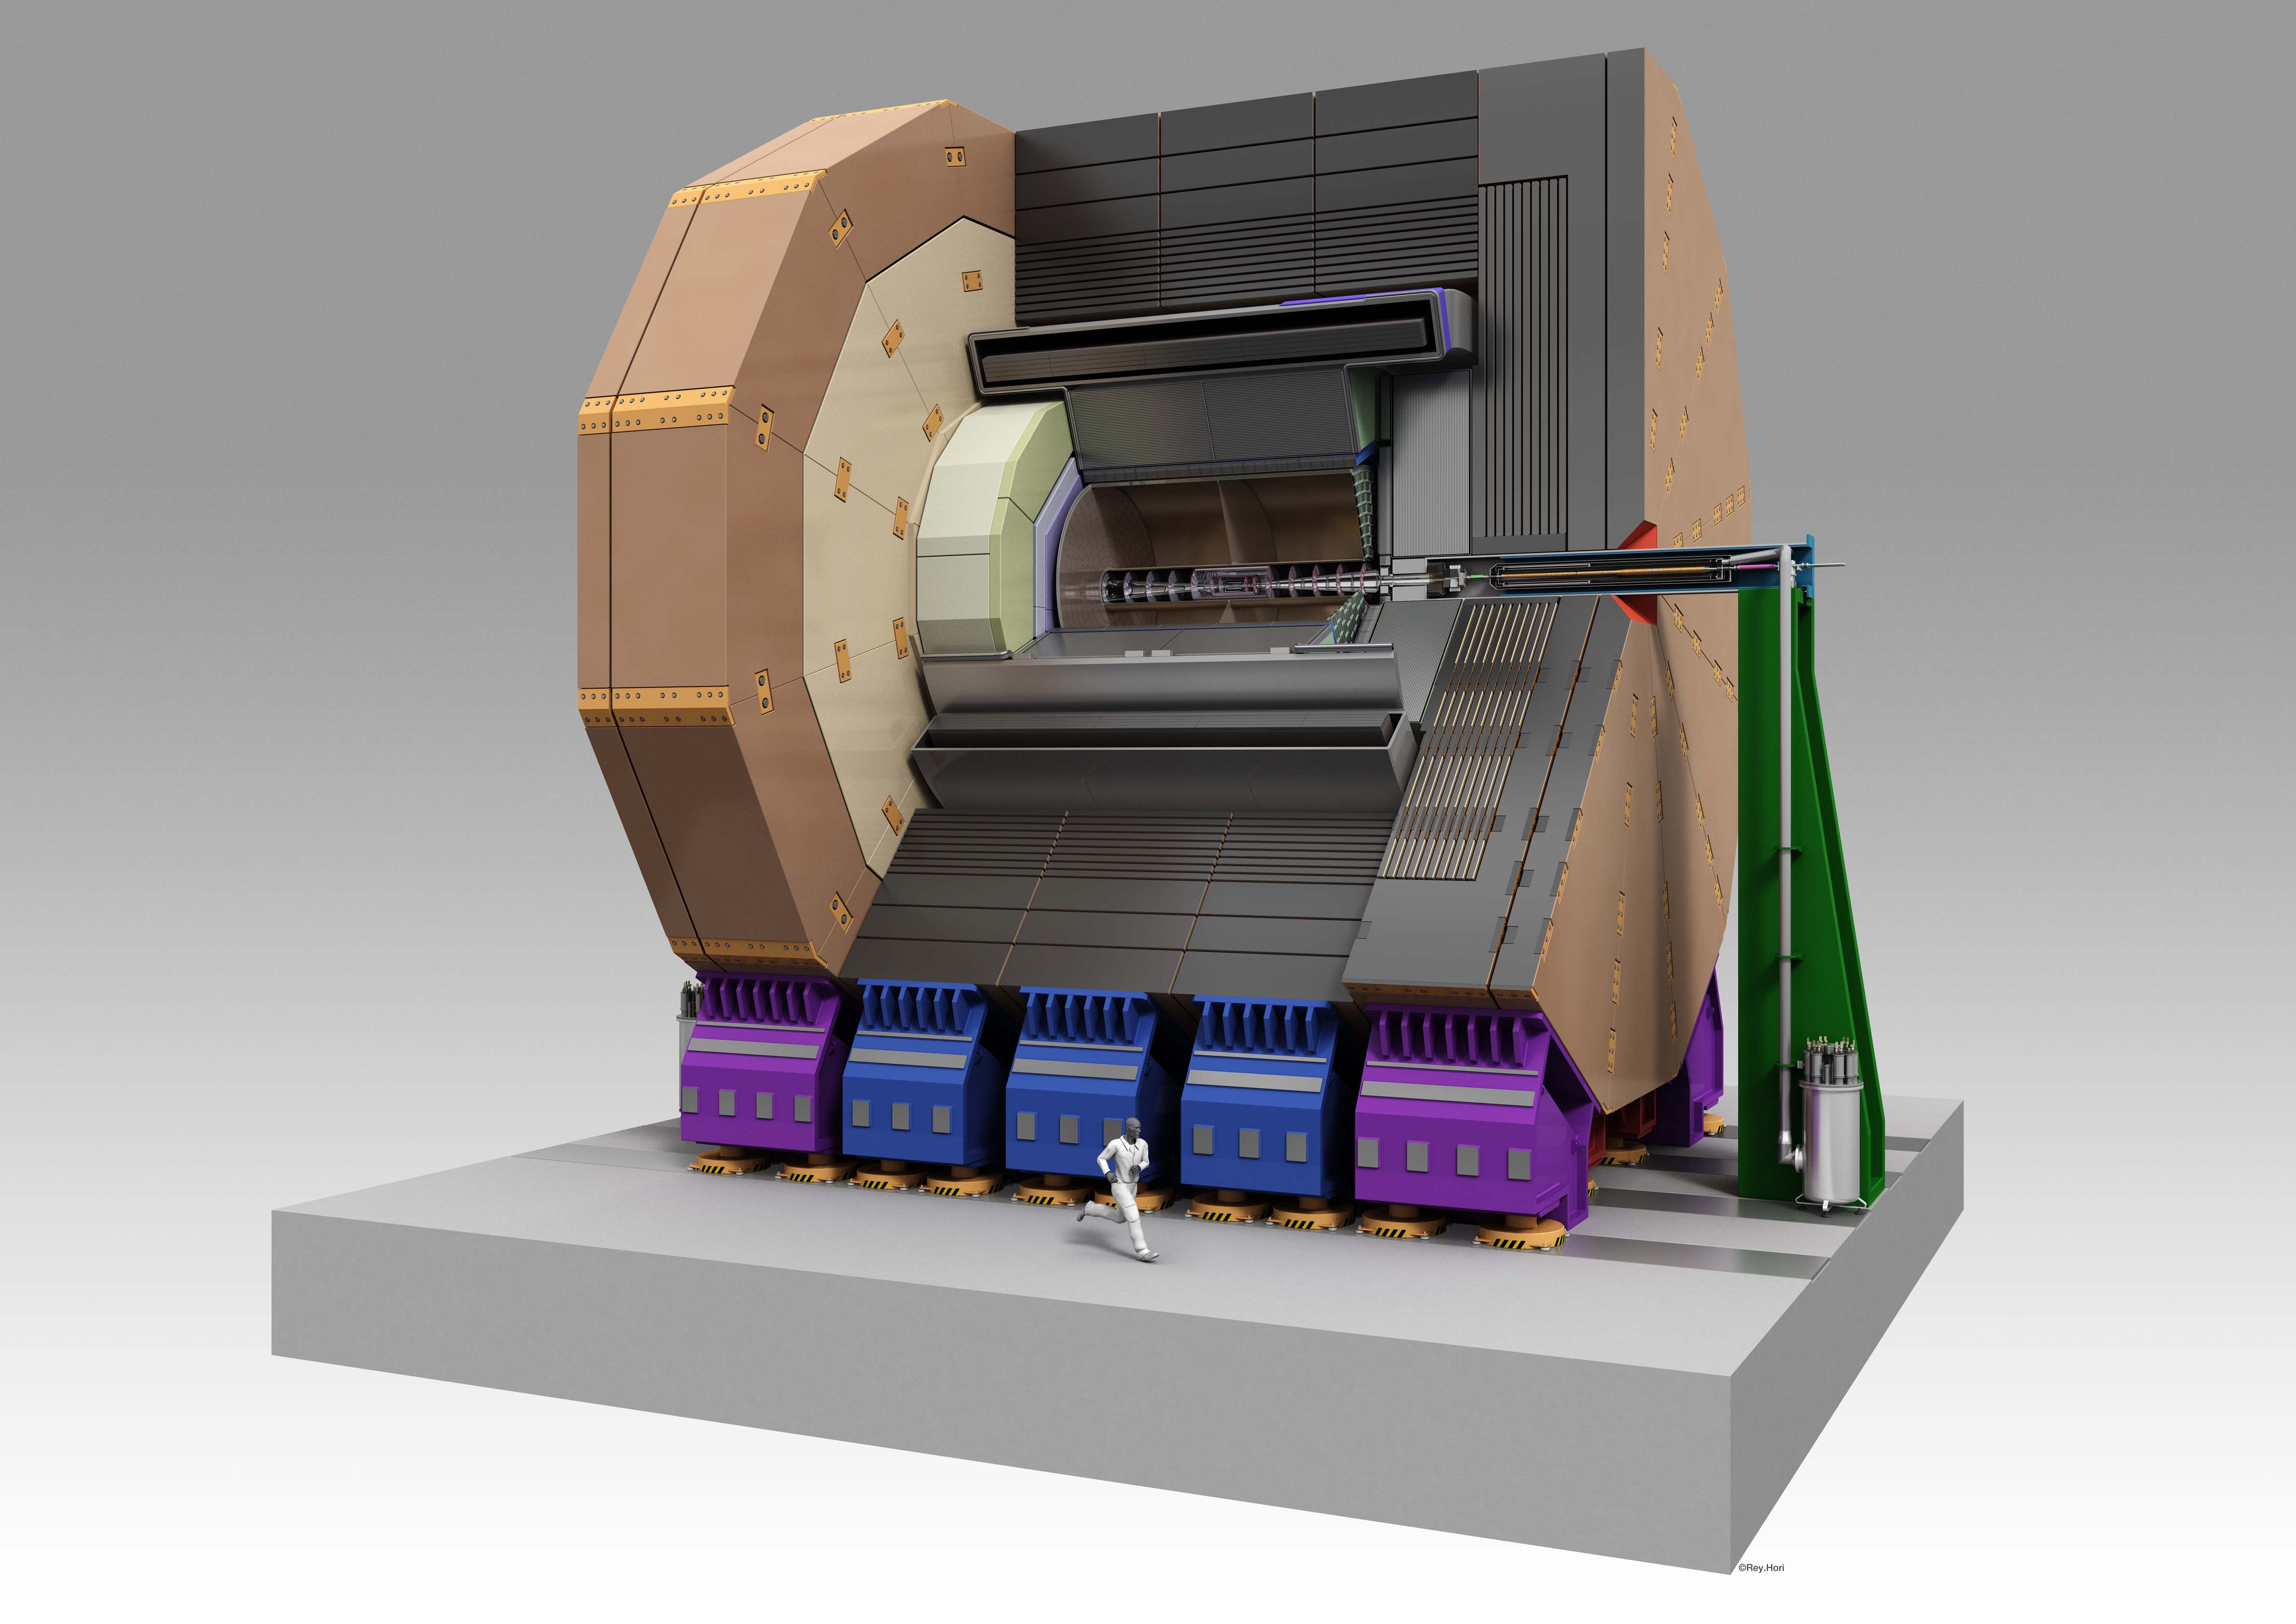
\includegraphics[width=0.5\textwidth]{LCDetectorsAndPFlow/Plots/Pictures/ILD_2.jpg}}
\caption[\protect\subref{fig:ild1} Quadrant view of the ILD detector concept.  The interaction point is in the lower right corner of the picture.  Dimensions are in mm.  \protect\subref{fig:ild2} View of the ILD detector concept.  Figures taken from  \cite{Behnke:2013lya}.]{\protect\subref{fig:ild1} Quadrant view of the ILD detector concept.  The interaction point is in the lower right corner of the picture.  Dimensions are in mm.  \protect\subref{fig:ild2} View of the ILD detector concept.  Figures taken from  \cite{Behnke:2013lya}.}
\label{fig:ild}
\end{figure} 

\subsection{Tracking System}
The tracking system for the ILD detector consist of a multi-layer pixel-vertex detector, which is surrounded by a system of silicon strip and pixel detectors.  These are purposed to give precise information about displaced vertices with respect to the impact point, which are crucial for the study of short lived particles such as the $D$ or $B$ mesons.  Outside of the vertex detector the central tracker of ILD, which is a Time Projection Chamber (TPC).  The TPC allows each charged particle track to be sampled at many space points giving precise information that can be used to extract the curvature of the track and the momentum of the charged particle transversing the track.  Finally, a further silicon strip detector surrounds the TPC to give an additional, high precision, space point to aid in the tracking performance. 

\subsubsection{Vertex System}
The main goal of the ILD vertex detector is to achieve a resolution on the impact parameter of charged particle tracks of $\sigma_{b} < 5 \oplus \frac{10}{p\text{sin}(\theta)^{3/2}} \mu$m, where the first term is the transverse impact parameters resolution and the second is a multiple-scattering term.  This makes it possible to precisely tag secondary vertices from charm and bottom mesons, which typically have relatively short proper lifetimes, $\tau$, such that $c\tau \approx \mathcal{O}(100-500) \mu$m.  To achieve this impact parameter resolution a spatial resolution of better than 3 {\mu}m is required near the IP will be required.  Furthermore, a low material budget of less than 0.15 \% $X_{0}$ per layer is needed to ensure that little energy is lost and that few electromagnetic showers are initiated within the tracker.  A low pixel occupancy will be essential for determining the trajectory of individual tracks in the detector.  The detector will have to be radiation hard to cope with the intense conditions found close to the IP due to the beam induced background, predominantly beamstrahlung.  Furthermore, consideration will have to be given as to the mechanical structure of the detector, power consumption and cooling.  

There are a number of different pixel technology options under consideration for the vertex detector for the ILD detector and this is an active area of ongoing research and development for the linear collider collaboration.  The current design of the vertex detector consists of three concentric layers of double-sided ladders that are close to being cylindrical.  Each ladder has two pixel sensors on each side and the ladder thickness is approximately 2 mm.  The inner most radii of the ladders ranges from 16 mm to 60mm from the IP.  In the simulation of the vertex detector silicon is used as the sensitive material and both support material and a cryostat is included for realism.  

\subsubsection{Silicon Tracking System}
There are four components that make up the silicon tracking system for ILD, shown in figure \ref{fig:vertex}.  These are the:

\begin{figure}
\centering
\subfloat[]{\label{fig:vertex1}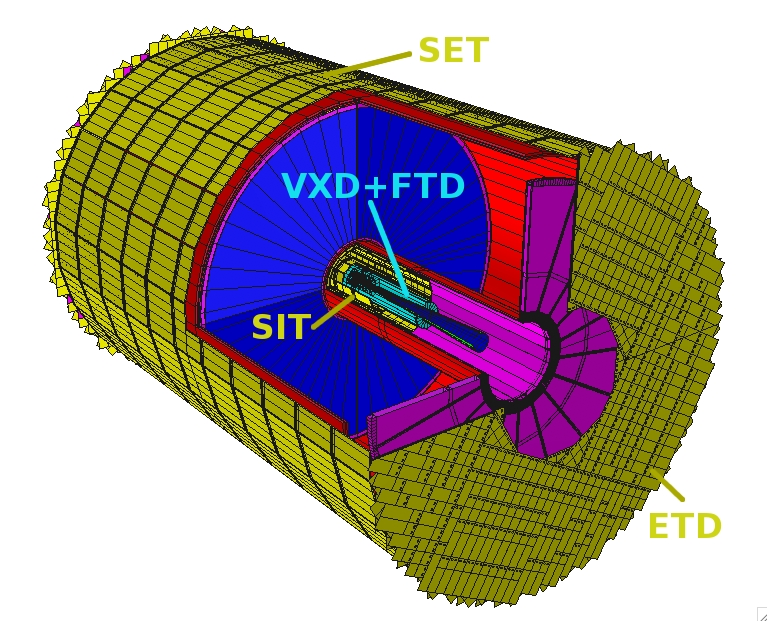
\includegraphics[width=0.5\textwidth]{LCDetectorsAndPFlow/Plots/Pictures/Vertex1.jpg}}
\subfloat[]{\label{fig:vertex2}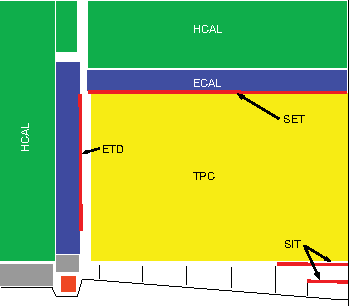
\includegraphics[width=0.5\textwidth]{LCDetectorsAndPFlow/Plots/Pictures/Vertex2.pdf}}
\caption[\protect\subref{fig:vertex1} A quadrant view of the ILD silicon envelope made of the four components SIT, SET, ETD and FTD as included in the full MOKKA simulation.  \protect\subref{fig:vertex2} a 3D detailed GEANT4 simulation description of the silicon system.  Figures taken from  \cite{Behnke:2013lya}.]{\protect\subref{fig:vertex1} A quadrant view of the ILD silicon envelope made of the four components SIT, SET, ETD and FTD as included in the full MOKKA simulation.  \protect\subref{fig:vertex2} a 3D detailed GEANT4 simulation description of the silicon system.  Figures taken from  \cite{Behnke:2013lya}.}
\label{fig:vertex}
\end{figure} 

\begin{itemize}
\item Silicon Inner Tracker (SIT) and Silicon External Tracker (SET).  These are both barrel components, which are positioned immediately inside and outside the TPC.  They act to provide additional space points that can be used in track fitting.  In particular these help to link the vertex detector with the TPC and help with extrapolation of TPC tracks into the calorimeter.  These silicon sensors will have a 50 {\mu}m pitch and will contain 200 m{\mu} thick silicon.  
\item Endplate of the TPC (ETD).  This sensor is identical to the SET, but is positioned in front of the ECal endcap calorimeter to extend the coverage of this silicon envelope. 
\item Forward tracker (FTD).  This detector consists of seven silicon disks, which extends the coverage of the tracking down to small angles which the TPC does not cover.  
\end{itemize}

The requirements for these sensors is similar to those of the vertex detector in terms of requiring low material budget and low occupancy, however, as the sensors are further away from the IP radiation hardness is less crucial.  The technology options for these sensors is also under development as was the case for the vertex detector.  In the detector model simulations all of these elements are included with additional material added to represent the support structure.  

\subsubsection{TPC}
The central tracking system for the ILD detector is a TPC, which is shown in figure \ref{fig:tracker}.  The TPC consists of two chambers of gas that has a high voltage applies across it.  Charged particles passing through the TPC ionise the gas and the ionised molecules drift in the high voltage to the end plates where they are collected and measured.  The drift time is then used to calculate the position of the ionisation point.  TPCs have the advantage over silicon tracking as they continuously track any charged particle passing through them unlike silicon detectors, which are only sensitive within the silicon layer.  This compensates for the worse single point resolution that TPCs have in comparison to a silicon detectors and makes TPCs a viable option for the ILD detector.  Furthermore, the TPC has a very low material budget, which benefits calorimetry in ILD.  The TPC will operate within a 3.5 T magnetic field and under these conditions a point resolution of better than 100 {\mu}m and a double hit resolution in $\phi$ of less than 2 mm can be achieved.  Several readout technology options that are dependent upon the gas mixture used for the TPC are currently under development.  For all potential options it is envisaged that the readout pads would be $\approx 1 \times 6 \text{mm}^{2}$ giving a total of approximately $10^{6}$ on the TPC endplates.

In the detector simulation the TPC is simulated as a cylindrical volume of the gas mixture, Ar:$\text{CH}_4$:$CO_{2}$ (95:3:2) \cite{Abe:2010aa}, which is surrounded by a realistic field cage.  Furthermore, a conservative estimate of the endplate is included in the simulation, which accounts for the support structure, electronics and cooling pipes.  Estimations have also been made for the material budget for power and readout cables that will serve the inner tracking detector.  These are included in the simulation as an aluminium cylinder between the beam pipe and the field cage of the TPC.

\begin{figure}
\centering
\subfloat[]{\label{fig:tracker1}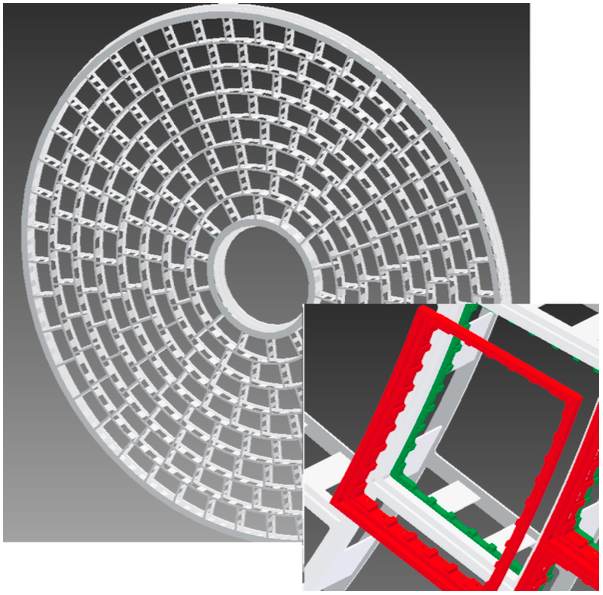
\includegraphics[width=0.5\textwidth]{LCDetectorsAndPFlow/Plots/Pictures/Tracker1.png}}
\subfloat[]{\label{fig:tracker2}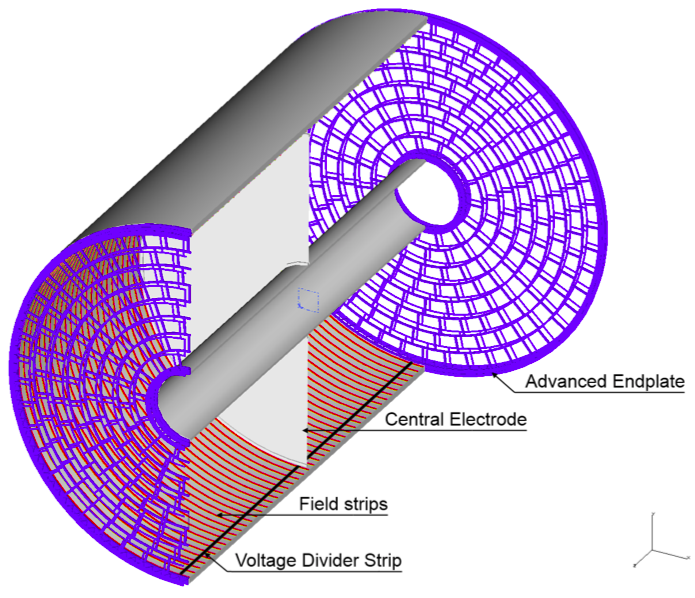
\includegraphics[width=0.5\textwidth]{LCDetectorsAndPFlow/Plots/Pictures/Tracker2.png}}
\caption[\protect\subref{fig:tracker1} Drawing of the propose end-plate for the TPC.  \protect\subref{fig:tracker2} Conceptual sketch of the TPC system showing the main parts of the TPC (not to scale).  Figures taken from  \cite{Behnke:2013lya}.]{\protect\subref{fig:tracker1} Drawing of the propose end-plate for the TPC.  \protect\subref{fig:tracker2} Conceptual sketch of the TPC system showing the main parts of the TPC (not to scale).  Figures taken from  \cite{Behnke:2013lya}.}
\label{fig:tracker}
\end{figure} 

\subsection{Electromagnetic Calorimeter}
A highly segmented electromagnetic sampling calorimeter (ECal) surrounds the ILD tracking system, which has been designed with particle flow calorimetry in mind.  To that extend the spatial resolution of particle showers within the ECal takes as much, if not more, precedence than the energy resolution.  The nominal ILD ECal is a silicon tungsten sampling calorimeter, which contains 30 layers and uses square cells with side length 5 mm, however, a scintillator strip option is also being considered.  

The primary goal of the ECal is to induce electromagnetic particles to shower within it and to record the energy deposited by those showers.  To that extent the ECal is constructed using tungsten as the absorber material.  As well as containing a large number of radiation lengths ($X_{0}$) per unit length, see table \ref{table:absorberoptions}, tungsten also has a small Moli�re radius and a large ratio of the radiation length to the nuclear interaction length.  The small Moli�re radius will lead to compact electromagnetic showers and make the separation of nearby showers easier, while the large ratio of the radiation length to nuclear interaction length will lead to greater longitudinal separation between electromagnetic and hadronic showers.  The use of tungsten in the nominal ILD ECal allows for a large number of radiation lengths, $\approx 24 X_{0}$, to be compacted within a relatively short distance, $\approx 20$ cm, which is sufficient for containing all but the highest energy electromagnetic showers.  The compact nature of the ECal also helps to reduce the overall size and cost of the detector.   A good energy resolution can be achieved with this configuration if 30 sampling layers are used.  The the tungsten thickness is 2.1mm for the inner 20 layers and 4.2mm for the last 10 layers to reduce the number of readout channels and cost, while maintaining a high sampling rate at the start of the calorimeter.  It should be noted that this offers no major gains in terms of energy resolutions in comparison to preexisting particle collider experiments \ref{Chatrchyan:2013dga, Perret:2014owa} because the focus of this calorimeter is split between imaging the particle showers and recording their energy as opposed to purely focusing on the energy measurement.  The 5 mm cell size for the ECal was chosen as a balance between being able to resolve nearby particle showers as well as reducing the overall cost of the calorimeter, which scales with the number of readout channels needed.  An optimisation study of the various ECal parameters for the ILD detector can be found in section \ref{sec:ecal}.

\begin{table}[h!]
\centering
\begin{tabular}{ l l l l l}
\hline
Material & $\lambda_{I}$ (cm) & $X_{0}$ (cm) & $\rho_{M}$ (cm) & $ \frac{\lambda_{I}}{X_{0}}$ \\
\hline
Fe & 16.8 & 1.76 & 1.69 & 9.5 \\
Cu & 15.1 & 1.43 & 1.52 & 10.6 \\
W & 9.6 & 0.35 & 0.93 & 27.4 \\
Pb & 17.1 & 0.56 & 1.00 & 30.5 \\
\hline
\end{tabular}
\caption[Comparison of the nuclear interaction length $\lambda_{I}$, radiation length $X_{0}$ and Moli�re radius for iron, copper, tungsten and lead.  Table taken from \cite{arXiv:0907.3577}.]{Comparison of the nuclear interaction length $\lambda_{I}$, radiation length $X_{0}$ and Moli�re radius for iron, copper, tungsten and lead.  Table taken from \cite{arXiv:0907.3577}.}
\label{table:absorberoptions}
\end{table}

As well as including the silicon tungsten sampling calorimeter, the simulation of the ILD ECal contains additional material to represent the instrumented region of the sensor and a heat shield as shown in figure \ref{fig:ecal}.

\begin{figure}
\centering
\subfloat[]{\label{fig:ecal1}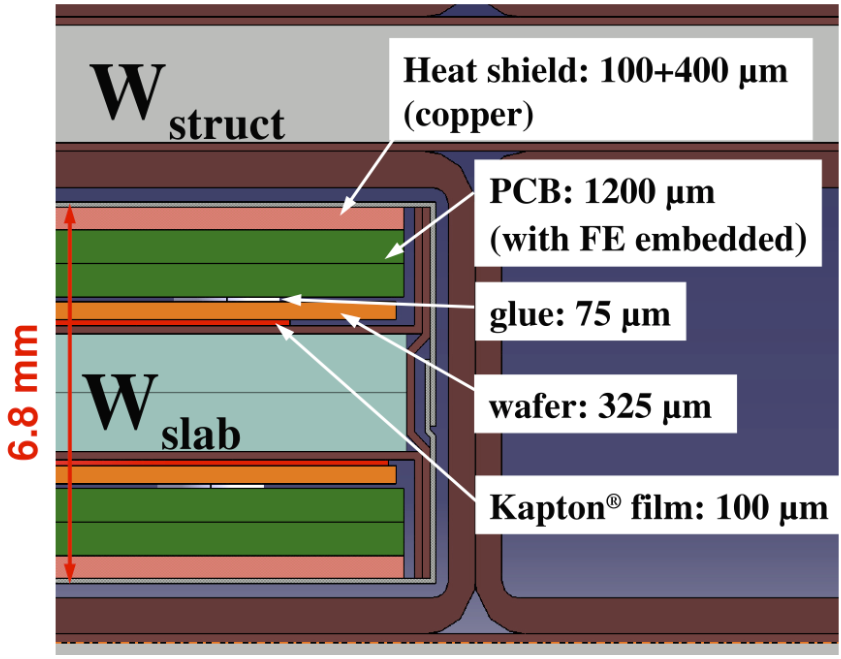
\includegraphics[width=0.4\textwidth]{LCDetectorsAndPFlow/Plots/Pictures/SiECal.png}} 
\hspace{1cm}
\subfloat[]{\label{fig:ecal2}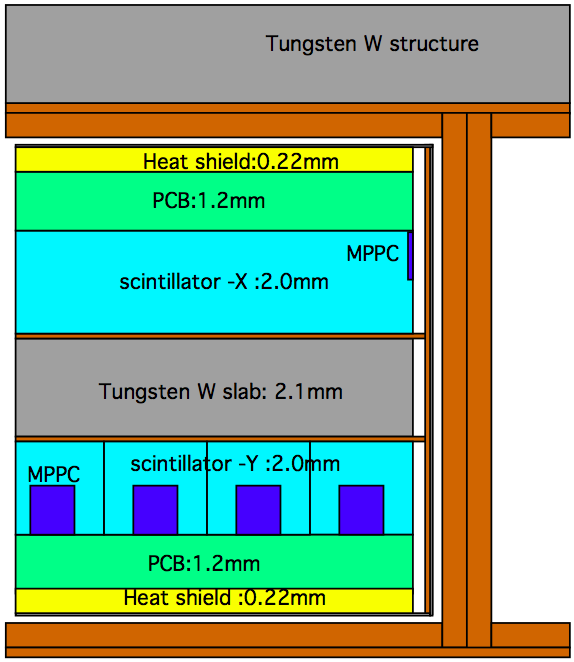
\includegraphics[width=0.4\textwidth]{LCDetectorsAndPFlow/Plots/Pictures/ScECal.png}}
\caption[Cross section through ECal layer for \protect\subref{fig:ecal1} silicon and \protect\subref{fig:ecal2} scintillator option.  Figures taken from  \cite{Behnke:2013lya}.]{Cross section through ECal layer for \protect\subref{fig:ecal1} silicon and \protect\subref{fig:ecal2} scintillator option.  Figures taken from  \cite{Behnke:2013lya}.}
\label{fig:ecal}
\end{figure} 

\subsection{Hadronic Calorimeter}
Surrounding the ECal is a finely segmented hadronic calorimeter (HCal), which has the primary goal of measuring the energy deposits from charged and neutral hadrons.  Similarly to the ECal the focus of this HCal is split between being able to resolve nearby particle showers and measuring their energy with a good resolution.  The nominal ILD HCal is a scintillator steel sampling calorimeter, which contains 48 layers and uses square cells with side length 30 mm.      
 
Iron is used as the absorber material for the HCal as it has excellent mechanical properties that allow the HCal to be constructed without auxiliary supports, which if required would act as dead regions in the detector.  Furthermore, iron is relatively inexpensive and given the nuclear interaction length is sufficiently small, it is possible to achieve a compact calorimeter design for low cost.  The relatively short radiation length found in iron is useful for fine sampling of the electromagnetic shower core that is found in hadronic showers, which exists due to the decays of $\pi^{0}$ and $\eta$ mesons.  This fine sampling leads to good energy resolution for the HCal for these shower components.  The nominal ILD HCal contains approximately $6 \lambda_{I}$, which when combined with the $1 \lambda_{I}$ in the ECal is sufficent for containing the majority of hadronic showers at ILC like energies.  The 48 layers are identical and are comprised of 20 mm of steel absorber with a 3 mm scintillator active medium.  The use of a square cell size of 30 mm is again a balance between reducing the cost of the detector, which is proportional to the number of readout channels and thus wants to lower the cell size, and achieving the required spatial resolution to make particle flow calorimetry possible.  Overall, the segmentation of the ILD HCal is able to give excellent spatial and energy resolution that can make particle flow a reality.  An optimisation study of the various HCal parameters for the ILD detector can be found in section \ref{sec:hcal}.

Simulation of the ILD HCal has a number of realistic features including detailed modelling of the electronics, detector gaps and the implementation of Birk's law for the scintillator sensitive detector elements.

\subsection{Forward Calorimetry}

Three additional sampling calorimeters are envisaged for the linear collider, LumiCal, LHCal and BeamCal, that will extend the coverage of the detector towards 4\pi and monitor the beam quality.  The LumiCal will aim to measure the luminosity with a precision of less than $10^{-3}$ at 500 GeV using Bhabha scattering, $\text{e}^{+}\text{e}^{-} \rightarrow \text{e}^{+}\text{e}^{-}(\gamma)$, as a gauge process \cite{Abe:2010aa}, while the BeamCal will make a bunch-bunch estimate of the luminosity and assist in the beam tuning.  Alongside the LumiCal is the LHCal, which extends the coverage of the HCal to low polar angle as shown in figure \ref{fig:fcal}.  The LumiCal covers polar angles between 31 and 77 mrad, while the BeamCal covers the range between 5 and 40 mrad.  The presence of beam-induced backgrounds along the beam line means these calorimeters will have to be radiation hard.  
 
\begin{figure}
\centering
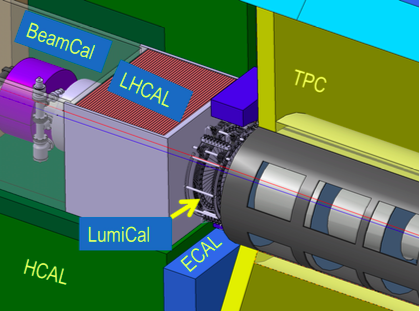
\includegraphics[width=0.5\textwidth]{LCDetectorsAndPFlow/Plots/Pictures/FCal.png}
\caption[The very forward revion of the ILD detector.  LumiCal, BeamCal and LHCal are carried by the support tube for the final focusing quadruple, QD0, and the beam pipe.  Figure taken from  \cite{Behnke:2013lya}.]{The very forward revion of the ILD detector.  LumiCal, BeamCal and LHCal are carried by the support tube for the final focusing quadruple, QD0, and the beam pipe.  Figure taken from  \cite{Behnke:2013lya}.}
\label{fig:fcal}
\end{figure} 

As the primary focus of these calorimeters is measuring the $\text{e}^{+}\text{e}^{-}$  beam, they are all constructed using tungsten absorber material to ensure narrow electromagnetic showers form within them.  The LumiCal layer configuration mirrors that of the ECal giving it a total of $\approx 24 X_{0}$ across its 30 layers.  Silicon is used as sensitive detector element for the LumiCal.  The LHCal uses silicon readout sensors identical to those found in the LumiCal and in total the LHCal contains $4 \lambda_{I}$ across 40 layers.  The BeamCal sensitive detector material is currently being developed as, due to the high occupancy from the beam induced backgrounds, a fast readout is required.  The cell sizes for these calorimeters is yet to be confirmed.  

In the context of particle flow calorimetry these calorimeters play a minimal role as few particles from the hard physics interaction will have their energy measured in these calorimeters and so they are not used in the reconstruction.

\subsection{Muon Chamber}
The ILD outer detector surrounds the HCal and is comprised of a coil, which generates a 3.5 T magnetic field, followed by an iron yoke.  The coil is one of the major cost drivers for the ILD detector and to minimise the size it does not encompass the iron yoke.  The yoke supplements measurements in the calorimeters by acting as a tail catcher for energy leaking out of the calorimeters and, furthermore, is used in the identification of muons.  The yoke is an iron scintillator sampling calorimeter, which consists of 10 layers spaced 14 cm apart followed by 2 (3) layers spaced 60 cm apart for the barrel (endcap) region of the detector as shown in figure \ref{fig:muon}.  There is also an additional sensitive layer for the barrel region placed immediately outside the HCal to help with association energy deposits between the calorimeters and the yoke.   

\begin{figure}
\centering
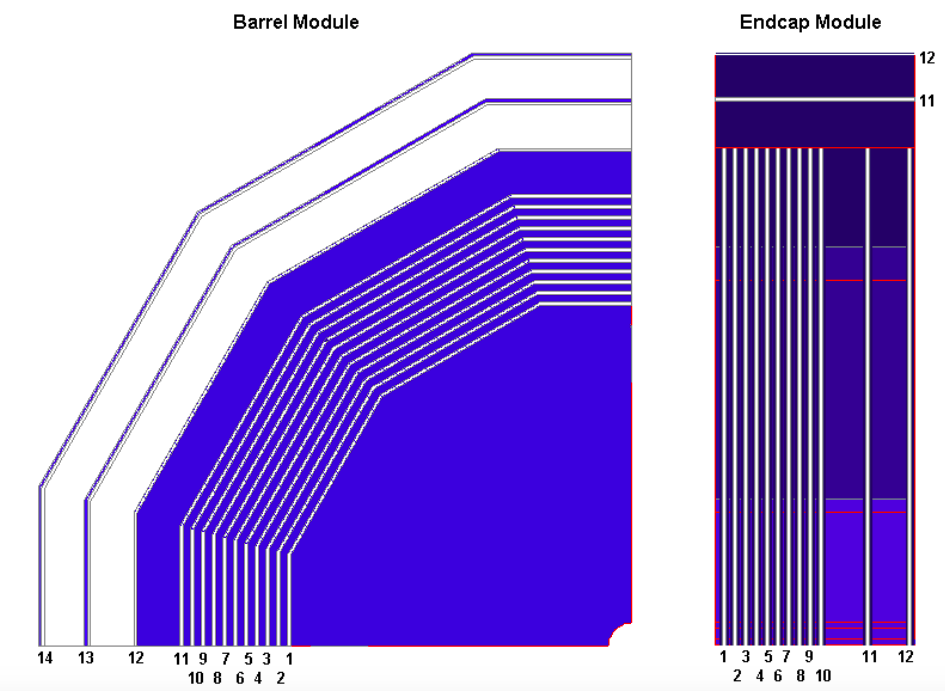
\includegraphics[width=0.5\textwidth]{LCDetectorsAndPFlow/Plots/Pictures/Muon.png}
\caption[The sensitive layers of the ILD muon system.  Figure taken from  \cite{Behnke:2013lya}.]{The sensitive layers of the ILD muon system.  Figure taken from  \cite{Behnke:2013lya}.}
\label{fig:muon}
\end{figure}   

The yoke uses scintillator strip readout technology and in the simulations a square cell size of 30 mm is assumed.  This is in contrast to the ILD baseline, which plans to use 3 cm wide and 1 m long strips, however, as the tail-catcher plays a minimal role in particle flow at ILC like energies this difference should have negligible impact.  

\subsection{CLIC ILD}
It is inappropriate to use the nominal ILD detector for simulations of the CLIC experiment due to the increased collision energy.  Therefore, the CLIC experiment has modified the nominal detector model to create a new detector model, CLIC\_ILD \cite{Linssen:2012hp} shown in figure \ref{fig:clicild}, which is more suited to CLIC like conditions.  The key differences between the nominal ILD detector and CLIC\_ILD  are:

\begin{itemize}
\item The higher energies found at the CLIC experiment lead to more intense beam induced backgrounds, which is especially problematic for detectors close to the IP where the occupancies will be extremely high.  To attempt to compensate for these effects the inner vertex detector in CLIC\_ILD is moved 15 mm further out from the IP.    
\item The HCal thickness is increased from 6 $\lambda_{I}$ to 7.5 $\lambda_{I}$.  This helps to contain the high energy particle showers found in the CLIC experiment to the calorimeters.
\item The HCal absorber material in the barrel is tungsten as opposed to iron.  This reduces the overall thickness of the HCal and keeps the coil size, one of the driving cost factors for the detectors, similar for the nominal ILD and CLIC\_ILD detectors.  In the endcaps iron is again used as the absorber material as there are no spatial requirements and it will lower the detector cost.  Furthermore, the shower development time in steel is faster than in tungsten making effective time stamping of energy deposits easier, which is crucial for the CLIC experiment for vetoing beam induced backgrounds.  
\item The magnetic field strength in the CLIC\_ILD detector is increased to 4 T.  This was found to benefit the reconstruction, particularly at high energies, as it leads to greater separation of charged particle tracks.  Furthermore, it was possible to achieve this increase in field strength using the nominal ILD coil design.   
\end{itemize}   

\begin{figure}
\centering
\subfloat[]{\label{fig:clicild1}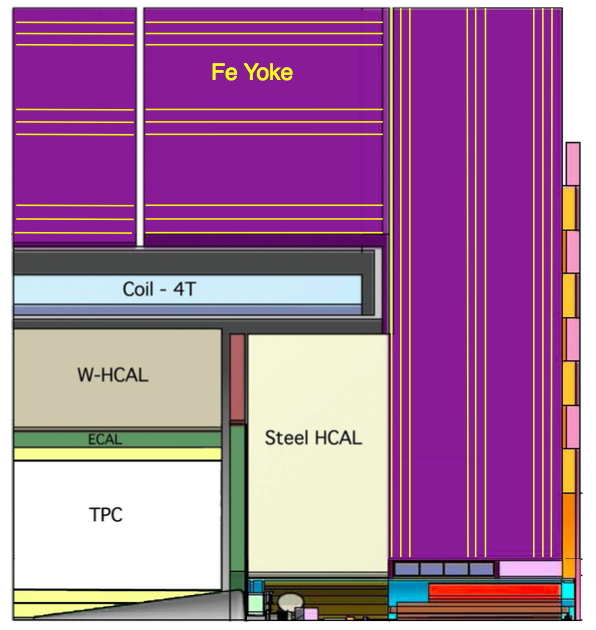
\includegraphics[width=0.5\textwidth]{LCDetectorsAndPFlow/Plots/Pictures/CLIC_ILD.png}}
\subfloat[]{\label{fig:clicild2}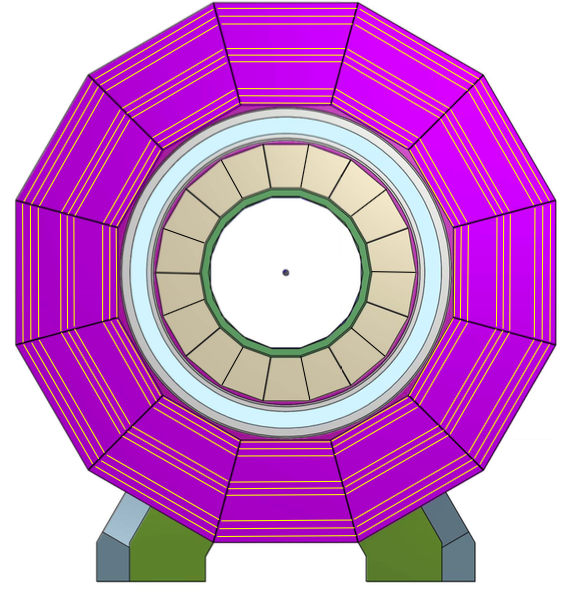
\includegraphics[width=0.5\textwidth]{LCDetectorsAndPFlow/Plots/Pictures/CLIC_ILD_2.png}}
\caption[\protect\subref{fig:ild1} Longitudinal (top quadrant) and \protect\subref{fig:ild2} transverse cross section of the CLIC\_ILD detector.  Figures taken from \cite{Linssen:2012hp}.]{\protect\subref{fig:ild1} Longitudinal (top quadrant) and \protect\subref{fig:ild2} transverse cross section of the CLIC\_ILD detector.  Figures taken from \cite{Linssen:2012hp}.}
\label{fig:clicild}
\end{figure} 

\section{PandoraPFA}

